% =====================================================================
% Figure 1: Conceptual diagram of mass-aware routing.
%
% Shows a packet acquiring mass as it traverses congested edges,
% causing the dynamic programming router to reroute it through
% cooler paths when its mass exceeds a viability threshold.
%
% Compile standalone:
%   pdflatex figure1_concept.tex
%
% Or include in main paper as:
%   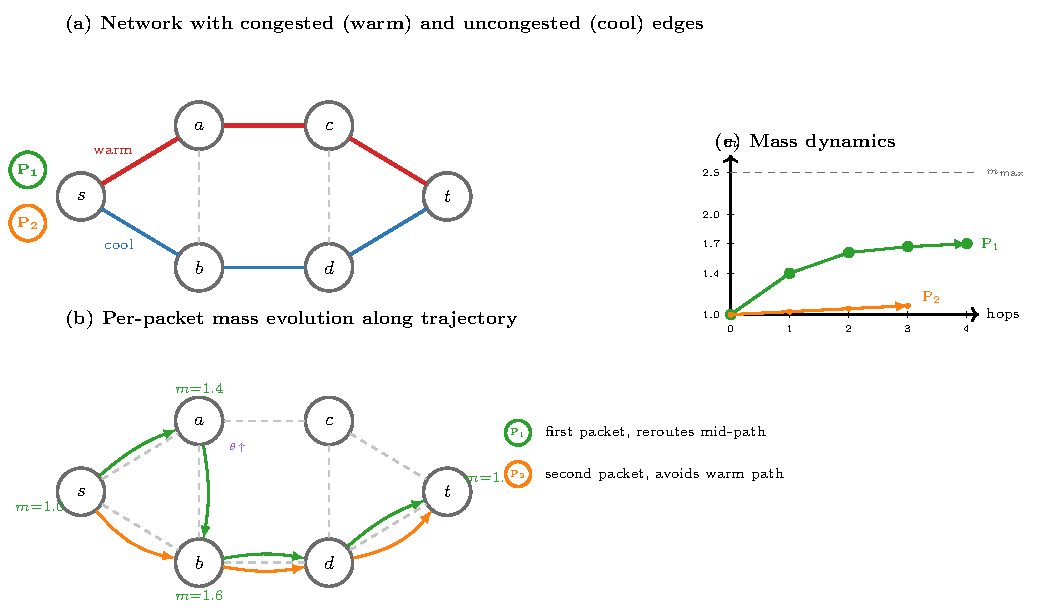
\includegraphics[width=\columnwidth]{figure1_concept}
% =====================================================================
\documentclass[tikz,border=4pt]{standalone}
\usepackage{amsmath, amssymb}
\usepackage{tikz}
\usetikzlibrary{positioning, arrows.meta, calc, decorations.pathmorphing,
                shapes.geometric, fit, backgrounds}

% --- Color palette (colorblind-safe + print-safe) ----------------------
\definecolor{coolblue}{HTML}{2E78B7}
\definecolor{warmred}{HTML}{D62728}
\definecolor{neutralgray}{HTML}{6C6C6C}
\definecolor{packetgreen}{HTML}{2CA02C}
\definecolor{packetorange}{HTML}{FF7F0E}
\definecolor{snapshotpurple}{HTML}{9467BD}

\tikzset{
  node n/.style = {circle, draw=neutralgray, very thick, fill=white,
                   minimum size=8mm, font=\small\bfseries, inner sep=0pt},
  edge cool/.style  = {coolblue,  line width=1.2pt},
  edge warm/.style  = {warmred,   line width=1.6pt},
  edge ghost/.style = {neutralgray!40, line width=0.8pt, dashed},
  packet/.style = {circle, draw, very thick, fill=white,
                   minimum size=6mm, font=\scriptsize\bfseries,
                   inner sep=0pt},
  packet1/.style = {packet, draw=packetgreen, text=packetgreen},
  packet2/.style = {packet, draw=packetorange, text=packetorange},
  arrow1/.style = {-{Latex[length=2mm]}, packetgreen,  line width=1pt},
  arrow2/.style = {-{Latex[length=2mm]}, packetorange, line width=1pt},
  panel label/.style = {font=\bfseries\small, anchor=north west},
  caption/.style = {font=\footnotesize, align=left, text width=8.5cm},
}

\begin{document}
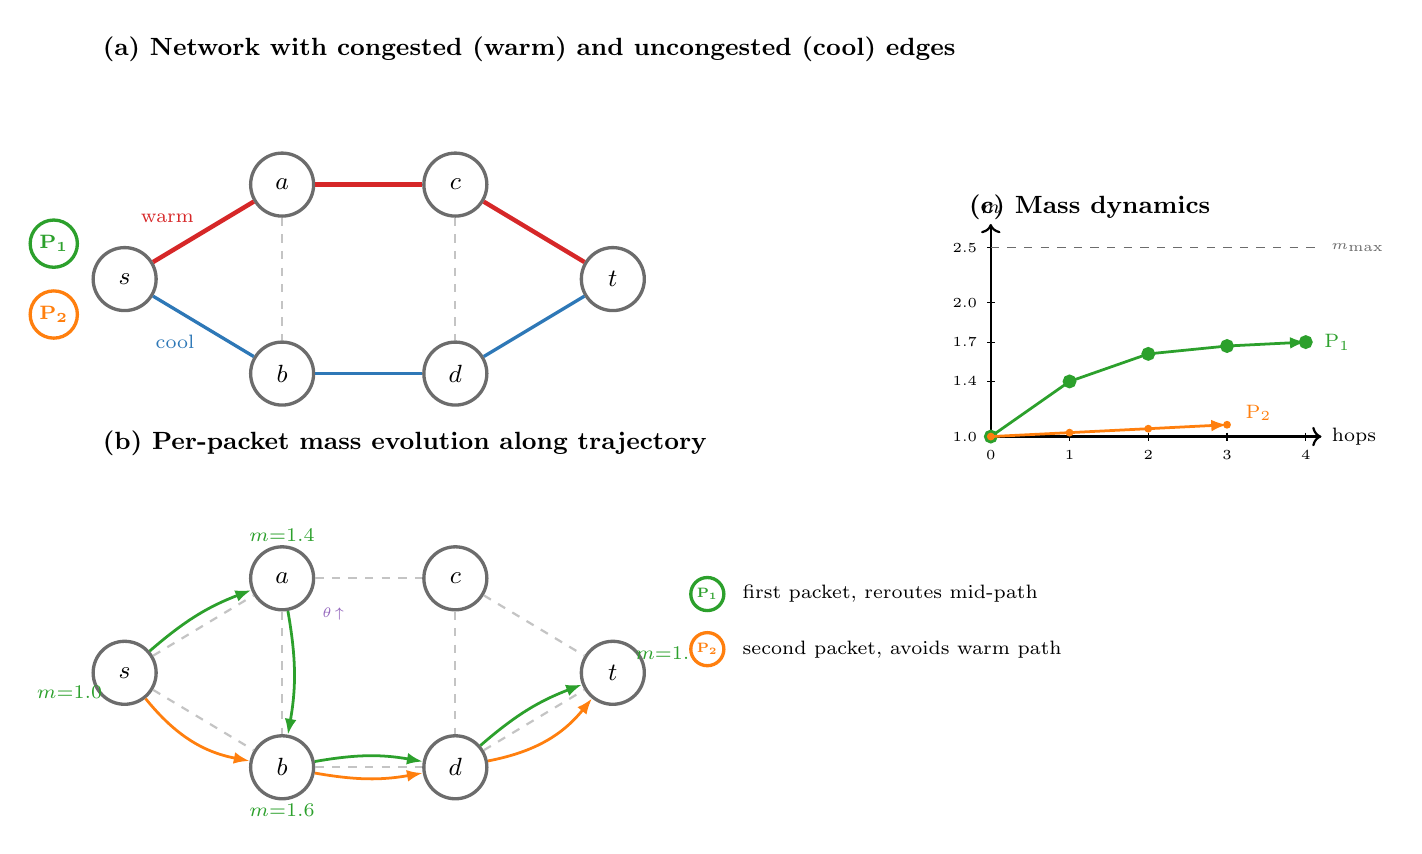
\begin{tikzpicture}

% =====================================================================
% PANEL (a) — Network topology with cool/warm edges
% =====================================================================
\begin{scope}[local bounding box=panela]
  \node[panel label] at (-0.4, 3.2) {(a) Network with congested (warm) and uncongested (cool) edges};

  % Six nodes
  \node[node n] (s)  at (0,    0)   {$s$};
  \node[node n] (a)  at (2,    1.2) {$a$};
  \node[node n] (b)  at (2,   -1.2) {$b$};
  \node[node n] (c)  at (4.2,  1.2) {$c$};
  \node[node n] (d)  at (4.2, -1.2) {$d$};
  \node[node n] (t)  at (6.2,  0)   {$t$};

  % Warm path: s -- a -- c -- t (congested, short)
  \draw[edge warm] (s) -- (a) node[midway, above left=-1pt, font=\scriptsize, warmred] {warm};
  \draw[edge warm] (a) -- (c);
  \draw[edge warm] (c) -- (t);

  % Cool path: s -- b -- d -- t (uncongested, longer in latency)
  \draw[edge cool] (s) -- (b) node[midway, below left=-1pt, font=\scriptsize, coolblue] {cool};
  \draw[edge cool] (b) -- (d);
  \draw[edge cool] (d) -- (t);

  % Cross link
  \draw[edge ghost] (a) -- (b);
  \draw[edge ghost] (c) -- (d);

  % Two packets at the source
  \node[packet1] at ($(s) + (-0.9,  0.45)$) {P\textsubscript{1}};
  \node[packet2] at ($(s) + (-0.9, -0.45)$) {P\textsubscript{2}};
\end{scope}

% =====================================================================
% PANEL (b) — Packet trajectories with mass growth
% =====================================================================
\begin{scope}[yshift=-5cm, local bounding box=panelb]
  \node[panel label] at (-0.4, 3.2) {(b) Per-packet mass evolution along trajectory};

  % Same node layout, slightly faded
  \node[node n] (s2)  at (0,    0)   {$s$};
  \node[node n] (a2)  at (2,    1.2) {$a$};
  \node[node n] (b2)  at (2,   -1.2) {$b$};
  \node[node n] (c2)  at (4.2,  1.2) {$c$};
  \node[node n] (d2)  at (4.2, -1.2) {$d$};
  \node[node n] (t2)  at (6.2,  0)   {$t$};

  % Faded edges as background
  \draw[edge ghost] (s2) -- (a2);
  \draw[edge ghost] (a2) -- (c2);
  \draw[edge ghost] (c2) -- (t2);
  \draw[edge ghost] (s2) -- (b2);
  \draw[edge ghost] (b2) -- (d2);
  \draw[edge ghost] (d2) -- (t2);
  \draw[edge ghost] (a2) -- (b2);
  \draw[edge ghost] (c2) -- (d2);

  % P1 trajectory: s -> a -> b -> d -> t  (starts on warm, reroutes)
  \draw[arrow1] (s2)  to[bend left=10]  (a2);
  \draw[arrow1] (a2)  to[bend left=10]  (b2);  % crosses to cool side
  \draw[arrow1] (b2)  to[bend left=10]  (d2);
  \draw[arrow1] (d2)  to[bend left=10]  (t2);

  % Mass annotations along P1
  \node[font=\scriptsize, packetgreen] at ($(s2)+(-0.7, -0.25)$)  {$m{=}1.0$};
  \node[font=\scriptsize, packetgreen] at ($(a2)+(0,    0.55)$)   {$m{=}1.4$};
  \node[font=\scriptsize, packetgreen] at ($(b2)+(0,   -0.55)$)   {$m{=}1.6$};
  \node[font=\scriptsize, packetgreen] at ($(t2)+(0.7,  0.25)$)   {$m{=}1.7$};

  % P2 trajectory: s -> b -> d -> t  (already cool because P1 left snapshot)
  \draw[arrow2] (s2) to[bend right=20] (b2);
  \draw[arrow2] (b2) to[bend right=10] (d2);
  \draw[arrow2] (d2) to[bend right=20] (t2);

  % Snapshot indicator near 'a' (where P1's transit raised loss snapshot)
  \node[snapshotpurple, font=\tiny\bfseries] at ($(a2)+(0.65,-0.45)$)
        {$\theta\!\uparrow$};

  % Legend
  \node[packet1, scale=0.7] (lp1) at (7.4, 1.0) {P\textsubscript{1}};
  \node[font=\scriptsize, anchor=west] at ($(lp1.east)+(0.1,0)$)
        {first packet, reroutes mid-path};
  \node[packet2, scale=0.7] (lp2) at (7.4, 0.3) {P\textsubscript{2}};
  \node[font=\scriptsize, anchor=west] at ($(lp2.east)+(0.1,0)$)
        {second packet, avoids warm path};
\end{scope}

% =====================================================================
% PANEL (c) — Mass vs hops curve
% =====================================================================
\begin{scope}[xshift=11cm, yshift=-2cm, local bounding box=panelc]
  \node[panel label] at (-0.4, 3.2) {(c) Mass dynamics};

  % Axes
  \draw[->, thick] (0,0) -- (4.2,0) node[right, font=\scriptsize] {hops};
  \draw[->, thick] (0,0) -- (0,2.7) node[above, font=\scriptsize] {$m$};

  % Axis ticks
  \foreach \x/\lab in {0/0, 1/1, 2/2, 3/3, 4/4} {
    \draw (\x,0.05) -- (\x,-0.05) node[below, font=\tiny] {\lab};
  }
  \foreach \y/\lab in {0/1.0, 0.7/1.4, 1.2/1.7, 1.7/2.0, 2.4/2.5} {
    \draw (0.05,\y) -- (-0.05,\y) node[left, font=\tiny] {\lab};
  }

  % m_max line
  \draw[dashed, neutralgray] (0,2.4) -- (4.2,2.4)
        node[right, font=\tiny, neutralgray] {$m_{\max}$};

  % P1 mass curve: 1.0 -> 1.4 -> 1.6 -> 1.65 -> 1.7
  \draw[arrow1, mark=*] plot coordinates {
    (0, 0)    % m=1.0
    (1, 0.7)  % m=1.4 (after warm edge)
    (2, 1.05) % m=1.6 (after cross-link, slightly hot)
    (3, 1.15) % m=1.65 (cool edge, tiny growth)
    (4, 1.2)  % m=1.7 (cool edge)
  };
  \foreach \x/\y in {0/0, 1/0.7, 2/1.05, 3/1.15, 4/1.2} {
    \filldraw[packetgreen] (\x,\y) circle (1.2pt);
  }

  % P2 mass curve: stays near 1.0 because cool path
  \draw[arrow2] plot coordinates {
    (0, 0)
    (1, 0.05)
    (2, 0.10)
    (3, 0.15)
  };
  \foreach \x/\y in {0/0, 1/0.05, 2/0.1, 3/0.15} {
    \filldraw[packetorange] (\x,\y) circle (1.2pt);
  }

  % Labels on curves
  \node[font=\scriptsize, packetgreen] at (4.4, 1.2) {P\textsubscript{1}};
  \node[font=\scriptsize, packetorange] at (3.4, 0.30) {P\textsubscript{2}};
\end{scope}

\end{tikzpicture}
\end{document}
